\subsection{2021年1月5日}
\paragraph{\href{https://www.51voa.com/VOA_Special_English/us-considers-vaccinating-more-people-using-half-doses-86059.html}{原文}}

\begin{figure}[H]
\centering
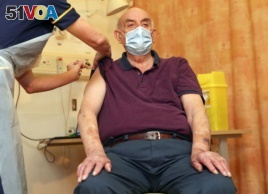
\includegraphics[scale=0.7]{003_voa_20210105.jpg}
\caption{82-year-old Brian Pinker receives the Oxford University-AstraZeneca COVID-19 vaccine from nurse Sam Foster at the Churchill Hospital in Oxford, southwest England on January 4, 2021.}
\end{figure}

By Susan Shand
04 January 2021
The United States says it is considering giving some people half the dose of Moderna's COVID-19 vaccine in order to vaccinate more people.
Moncef Slaoui is the head the country's vaccine program. He said Sunday that officials were discussing the possible plan with Moderna and the Food and Drug Administration (FDA). Moderna's vaccine requires two doses per individual.
He said that giving half of the dose to people between the ages of 18 and 55 will allow the vaccination program to "double the number of people with the doses we have."
He added that just one injection causes an "identical" immunity.
Moderna and the FDA could not immediately be reached for comment.
The U.S. Centers for Disease Control and Prevention said it had injected more than four million people with a first dose of vaccine by Monday morning. It said it had sent out more than 13 million doses.
The U.S. has also approved a two-dose vaccination treatment from drug company Pfizer.
The government's vaccination plan has not been meeting its goals. Officials had hoped to have 20 million people vaccinated by the end of the 2020.
Vaccine race
Britain has administered about one million vaccinations since it approved the Pfizer vaccine in early December. On Monday, it became the first country to use a vaccine developed by Oxford University and AstraZeneca. That vaccine is easier to store and transport.
A new surge of COVID-19 cases is threatening the country's National Health Service. Britain is trying to vaccinate older people and others at higher risk from the disease. Prime Minister Boris Johnson's government has secured 100 million doses of the Oxford/AstraZeneca vaccine.
Eighty-two-year-old Brian Pinker was the first person to get that vaccine outside of experimental use.
Pinker, who has kidney disease, said he was "proud" the medicine was invented in Oxford.
Israel is the world's vaccination leader. More than ten percent of its population is already vaccinated. Israel is now injecting more than 150,000 people a day.
In December 2020, China approved its first COVID-19 vaccine. It is one injection and was created by drugmaker Sinopharm. The government-owned company has said its treatment is 79 percent effective against the virus.
Russia has been providing its COVID-19 vaccine, called Sputnik V, since August. More than 100,000 people have been injected. In November, the government said the treatment was more than 91 percent effective.
New versions
Britain has seen a surge in coronavirus cases in recent weeks as officials struggle to control the spread of a new version of the COVID-19 virus. The new version is far more contagious than others. Officials have recorded more than 50,000 new infections a day since December 29. On Monday, they reported 407 deaths related to the virus. That brings the total number of confirmed COVID deaths in Britain to 75,431.
Britain also reports the presence of a second new version of coronavirus. It appears that version came from South Africa.
Johnson said on Sunday that more restrictions were likely, even with millions already living under the highest level of restrictions.
Starting at midnight tonight, most of mainland Scotland will be in total lockdown, announced Scottish First Minister Nicola Sturgeon.
Europe
In Germany, government spokesman Steffen Seibert said Monday that the government does not regret its decision last year to have the European Union order vaccines for all 27 nations. He said that for a country in the middle of Europe with many borders, "everyone for themselves cannot be the way."
Nearly 265,000 vaccinations have been reported since the program began one week ago. Critics are pointing to faster programs in the U.K., the U.S. and Israel.
Health Ministry spokesman Hanno Kautz said 1.3 million doses of the BioNTech-Pfizer vaccine were delivered to Germany before the end of 2020 and another 670,000 are due on Friday. Germany has 83 million people.
I'm Susan Shand.
The Associated Press and the Reuters News Agency reported this story. Susan Shand adapted it for Learning English. Caty Weaver was the editor.

\begin{messagebox}
Words in This Story
dose – n. the amount of a medicine, drug, or vitamin that is taken at one time
immunity – n. the power to keep yourself from being affected by a disease
surge - n. a move that is very quick and sudden in a particular direction
contagious – adj. able to be passed from one person or animal to another by touching
\end{messagebox}

The United States says it is considering giving some people half the dose of Moderna's COVID-19 vaccine in order to vaccinate more people.
美国称其正考虑给某些人接种一半剂量的新冠肺炎疫苗,以便为更多人接种疫苗。
Moncef Slaoui is the head the country's vaccine program. He said Sunday that officials were discussing the possible plan with Moderna and the Food and Drug Administration (FDA). Moderna's vaccine requires two doses per individual.
蒙塞夫·斯拉维是美国疫苗项目的负责人。他周日表示,有关官员正同莫德纳公司以及美国食品药品管理局讨论这种可能的方案。莫德纳公司的疫苗需要每人注射两针。
He said that giving half of the dose to people between the ages of 18 and 55 will allow the vaccination program to "double the number of people with the doses we have."
他说,给年龄在18到55岁之间的人士注射一半剂量的疫苗,将使疫苗接种计划能够将“现有疫苗的可接种人数翻倍。”
He added that just one injection causes an "identical" immunity.
他还表示,只注射一针剂量会产生“完全相同”的免疫效果。
Moderna and the FDA could not immediately be reached for comment.
莫德纳公司和美国食品药品管理局未能立即发表评论。
The U.S. Centers for Disease Control and Prevention said it had injected more than four million people with a first dose of vaccine by Monday morning. It said it had sent out more than 13 million doses.
美国疾病控制预防中心表示,截至周一早上,已经向超过400万人注射了第一针疫苗。该中心称其已经发放了超过1300万剂疫苗。
The U.S. has also approved a two-dose vaccination treatment from drug company Pfizer.
美国还批准了辉瑞制药公司的一种两剂疫苗疗法。
The government's vaccination plan has not been meeting its goals. Officials had hoped to have 20 million people vaccinated by the end of the 2020.
美国政府的疫苗方案尚未达成其目标。官员们希望在2020年底前接种2000万人。
Vaccine race
疫苗竞赛
Britain has administered about one million vaccinations since it approved the Pfizer vaccine in early December. On Monday, it became the first country to use a vaccine developed by Oxford University and AstraZeneca. That vaccine is easier to store and transport.
英国自12月初批准辉瑞疫苗以来,已经进行了大约100万次接种。英国周一成为采用牛津大学和阿斯利康公司所研发疫苗的首个国家。这种疫苗更易于储存和运输。
A new surge of COVID-19 cases is threatening the country's National Health Service. Britain is trying to vaccinate older people and others at higher risk from the disease. Prime Minister Boris Johnson's government has secured 100 million doses of the Oxford/AstraZeneca vaccine.
新一轮的新冠肺炎病例正在威胁该国的国民医疗服务体系。英国正尝试给老年人和其它高风险人群接种。英国首相鲍里斯·约翰逊领导的政府已经获得了1亿剂牛津大学和阿斯利康公司研发的疫苗。
Eighty-two-year-old Brian Pinker was the first person to get that vaccine outside of experimental use.
82岁的布莱恩·平克是实验用途之外接种该疫苗的第一人。
Pinker, who has kidney disease, said he was "proud" the medicine was invented in Oxford.
患有肾脏疾病的平克表示,他对牛津大学研发的这种药物感到骄傲。
Israel is the world's vaccination leader. More than ten percent of its population is already vaccinated. Israel is now injecting more than 150,000 people a day.
以色列是全球疫苗接种的领跑者。该国10\%以上人口已经接种了疫苗。以色列现在每天给超过15万人注射疫苗。
In December 2020, China approved its first COVID-19 vaccine. It is one injection and was created by drugmaker Sinopharm. The government-owned company has said its treatment is 79 percent effective against the virus.
2020年12月,中国批准了该国第一种新冠肺炎疫苗。它是由国药集团生产的一种注射剂。这家国有企业称其疫苗对新冠病毒的有效率为79\%。
Russia has been providing its COVID-19 vaccine, called Sputnik V, since August. More than 100,000 people have been injected. In November, the government said the treatment was more than 91 percent effective.
俄罗斯自8月份以来一直在接种一种名为Sputnik V的新冠肺炎疫苗。已经有超过10万人接种。俄罗斯政府在11月表示,该疫苗的有效率为91\%以上。
New versions
病毒新变种
Britain has seen a surge in coronavirus cases in recent weeks as officials struggle to control the spread of a new version of the COVID-19 virus. The new version is far more contagious than others. Officials have recorded more than 50,000 new infections a day since December 29. On Monday, they reported 407 deaths related to the virus. That brings the total number of confirmed COVID deaths in Britain to 75,431.
由于官员们难以控制一种新冠病毒变种的传播,英国近几周新冠病毒病例激增。这种新变种比其它类型病毒的感染力更强。自12月29日以来,官方每天录得超过5万例新增感染病例。周一,英国报告了407例与这种病毒有关的死亡病例。这使得英国确诊新冠肺炎死亡总人数达到了75431人。
Britain also reports the presence of a second new version of coronavirus. It appears that version came from South Africa.
英国还报告出现了第二种新冠病毒变种。这种新变种病毒似乎来自于南非。
Johnson said on Sunday that more restrictions were likely, even with millions already living under the highest level of restrictions.
约翰逊周日表示可能会出台更多限制措施,即便已经有数百万人生活在最高级别的限制措施之下。
Starting at midnight tonight, most of mainland Scotland will be in total lockdown, announced Scottish First Minister Nicola Sturgeon.
苏格兰首相尼古拉·斯特金宣布,从今晚午夜开始,苏格兰大部分地区将处于全面封锁状态。
Europe
欧洲
In Germany, government spokesman Steffen Seibert said Monday that the government does not regret its decision last year to have the European Union order vaccines for all 27 nations. He said that for a country in the middle of Europe with many borders, "everyone for themselves cannot be the way."
在德国,政府发言人斯坦芬·塞伯特周一表示,德国政府对去年决定为欧盟所有27个成员国订购疫苗的决定不感后悔。他说,对于一个处于欧洲中部、边界众多的国家来说,“人人只想着自己不是解决办法。”
Nearly 265,000 vaccinations have been reported since the program began one week ago. Critics are pointing to faster programs in the U.K., the U.S. and Israel.
自一周前该计划开始以来,已经报告有近26.5万人接种。批评人士指出英国、美国和以色列推出了更快的疫苗接种计划。
Health Ministry spokesman Hanno Kautz said 1.3 million doses of the BioNTech-Pfizer vaccine were delivered to Germany before the end of 2020 and another 670,000 are due on Friday. Germany has 83 million people.
德国卫生部发言人汉诺·考茨表示,2020年底前已经向德国交付了130万剂由BioNTech和辉瑞公司联合研制的疫苗,周五还将会交付67万剂疫苗。德国有8300万人口。
